% Reviewer-facing replacement for the numerical-experiments section.
% Required packages: amsmath, booktabs, graphicx, and xcolor.
% Figure paths are relative to this file's directory.

\begingroup
\color{blue}

\section{Numerical Experiments}
\label{sec:numerical-experiments}

We evaluate Transductively Standardized Conformal Prediction (TSCP) on
simulated and real multivariate regression problems. The experiments are
organized around four questions. First, does TSCP retain joint marginal
coverage while adapting the interval length of each outcome coordinate?
Second, is the conclusion stable under dependence and partial
heteroskedasticity? Third, does the advantage persist with quantile-regression
scores and against CQHR? Finally, what is the observed wall-clock cost of the
construction? Additional sensitivity analyses, including heavy tails,
contamination, and a convex shape-template baseline, are reported in
Appendix~\ref{app:additional-experiments}.

\subsection{Methods and Evaluation Metrics}
\label{sec:experiment-methods}

The primary comparisons use four methods. \emph{Unscaled Max} applies split
conformal prediction to the maximum coordinate-wise residual. \emph{Point
CHR} estimates coordinate scales using an additional data split. \emph{Emp.
Copula} estimates a dependence model from the calibration residuals and then
uses the same observations for calibration; this implementation does not have
the finite-sample guarantee enjoyed by the other methods. \emph{TSCP} denotes
the rectangular local-worst-case construction proposed in this paper. For
quantile-regression experiments, we additionally compare with the native CQHR
method of Sampson and Chan (2024). Appendix~\ref{app:shape-template} contains a
separate low-dimensional comparison with the hyperrectangular shape-template
method of Tumu et al. (2024).

For a test sample of size $m$, we report the empirical joint coverage
\[
  \widehat{\operatorname{Cov}}
  = \frac{1}{m}\sum_{i=1}^{m}
    \mathbf{1}\!\left\{\boldsymbol{Y}_i
    \in \widehat{C}(\boldsymbol{X}_i)\right\}.
\]
For absolute residual scores, all methods return a rectangle with residual
half-widths $(L_1,\ldots,L_d)$. We therefore report the normalized
residual-space volume $\prod_{j=1}^{d}L_j$, which equals $2^{-d}$ times the
full rectangular volume, and the full coordinate-wise interval lengths
$2L_j$. For CQR, the base interval depends on the test covariates, so volume
and coordinate lengths are averaged in the original outcome space. Runtime is
the wall-clock time needed to construct the conformal region after residuals
have been computed; fitting the common regression model is excluded. Unless
stated otherwise, absolute-residual results are averaged over 200 repetitions
and the target coverage is $1-\alpha=0.9$. Every synthetic repetition redraws
independent training, test, and calibration observations while holding the
underlying regression coefficients fixed. The figures show mean curves
without error bars; across-repetition standard deviations and an uncertainty
audit are reported in Appendix~\ref{app:coverage-uncertainty} and the
accompanying CSV files.

\subsection{Absolute-Residual Experiments}
\label{sec:absolute-residual-experiments}

We first generate $10$-dimensional features
$\boldsymbol{X}\sim\mathcal{N}(\boldsymbol{0},I_{10})$ and outcomes
\[
  Y_j = f_j(\boldsymbol{X}) + \epsilon_j,
  \qquad j\in[10],
\]
where every $f_j$ is linear and the nonzero coefficients are sampled once
from $\operatorname{Unif}(-10,10)$. Each repetition independently draws 7,200
observations to fit ordinary least squares, 800 test observations, and a
separate calibration sample of size
$n\in\{30,50,100,300,500\}$.

\paragraph{Heterogeneous and dependent noise.}
The first experiment uses
$\boldsymbol{\epsilon}\sim\mathcal{N}(\boldsymbol{0},DRD)$, where
$D=\operatorname{diag}(10,9,\ldots,1)$ and $R$ is equicorrelated with
$\rho=0.6$. This simultaneously tests heterogeneous coordinate scales and
cross-output dependence. Figure~\ref{fig:body-abs-overview} reports joint
coverage, residual-space volume, construction time, and coordinate-wise
lengths. At $n=100$, TSCP attains coverage $0.907$ with average volume
$3.57\times10^{10}$, compared with coverage $0.904$ and volume
$5.24\times10^{10}$ for Point CHR. Unscaled Max has coverage $0.902$ but a
volume of $7.42\times10^{12}$. Emp. Copula is smaller but undercovers, with
coverage $0.873$.

\begin{figure*}[t]
  \centering
  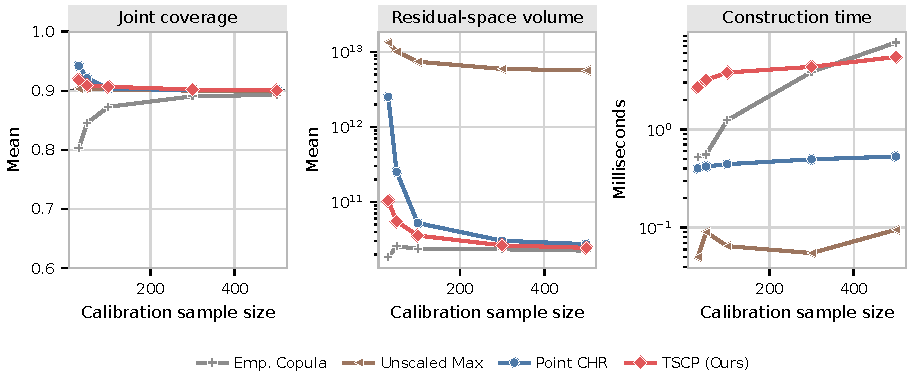
\includegraphics[width=0.94\textwidth]{figures/fig_body_abs_residual_overview.pdf}
  \caption{Absolute-residual experiment with $d=10$, heterogeneous Gaussian
  scales $(10,9,\ldots,1)$, and equicorrelation $\rho=0.6$. Curves report
  averages over 200 repetitions; the dashed line marks the target joint
  coverage. Runtime excludes the common model fit.}
  \label{fig:body-abs-overview}
\end{figure*}

Figure~\ref{fig:body-abs-coordinate-bars} makes the dimension-specific
behavior explicit at $n=100$. The mean TSCP full interval length decreases
from $49.4$ on the noisiest coordinate to $5.0$ on the quietest coordinate.
In contrast, Unscaled Max assigns the same length, approximately $38.0$, to
every coordinate. Thus, similar overall coverage does not imply similar
marginal informativeness: TSCP allocates width according to coordinate scale
instead of allowing the noisiest output to determine all ten intervals. The
smaller Emp. Copula bars must be read together with its joint undercoverage in
Figure~\ref{fig:body-abs-overview}.

\begin{figure*}[t]
  \centering
  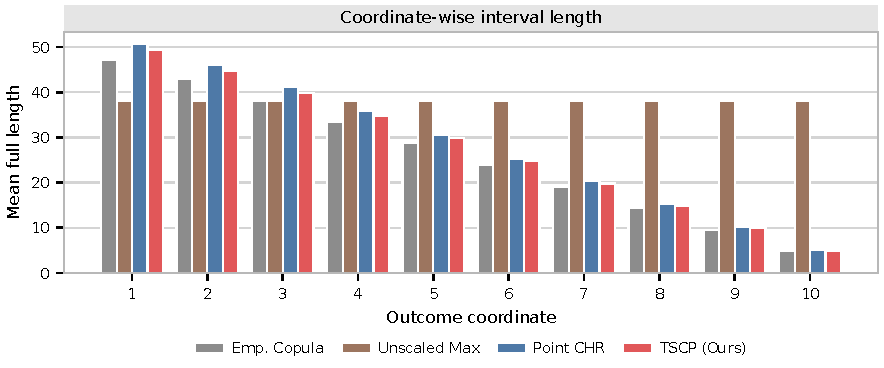
\includegraphics[width=0.90\textwidth]{figures/fig_body_abs_coordinate_bars.pdf}
  \caption{Coordinate-wise mean full interval lengths for the
  absolute-residual experiment with $d=10$, $n=100$, heterogeneous Gaussian
  scales $(10,9,\ldots,1)$, and equicorrelation $\rho=0.6$. Residual-space
  half-widths are multiplied by two to report full outcome intervals. Results
  average 200 independent repetitions.}
  \label{fig:body-abs-coordinate-bars}
\end{figure*}

\paragraph{Partial heteroskedasticity.}
To distinguish heterogeneity across coordinates from heteroskedasticity with
respect to the input, we next make only the first five coordinates
heteroskedastic. For $j\leq5$, conditional on $X_1=x_1$, the noise standard
deviation is
\[
  \sigma_j(x_1)
  = (11-j)\sqrt{\frac{1+1.5x_1^2}{2.5}},
\]
while $\sigma_j(x_1)=11-j$ for $j>5$. The normalization preserves
$\mathbb{E}[\sigma_j^2(X_1)]=(11-j)^2$, so the comparison isolates
input-dependent variance rather than changing the marginal second moments.

Figure~\ref{fig:body-partial-hetero} shows that TSCP remains close to the
target across calibration sizes and continues to adapt coordinate-wise. At
$n=100$, TSCP obtains coverage $0.904$ and average volume
$1.40\times10^{11}$; Point CHR obtains coverage $0.902$ and volume
$2.94\times10^{11}$, while Unscaled Max obtains coverage $0.900$ and volume
$2.33\times10^{13}$. This is a marginal-coverage experiment. It does not
assert conditional coverage at each value of $X_1$, nor does the present
global coordinate standardization attempt to estimate the local variance
function.

\begin{figure*}[t]
  \centering
  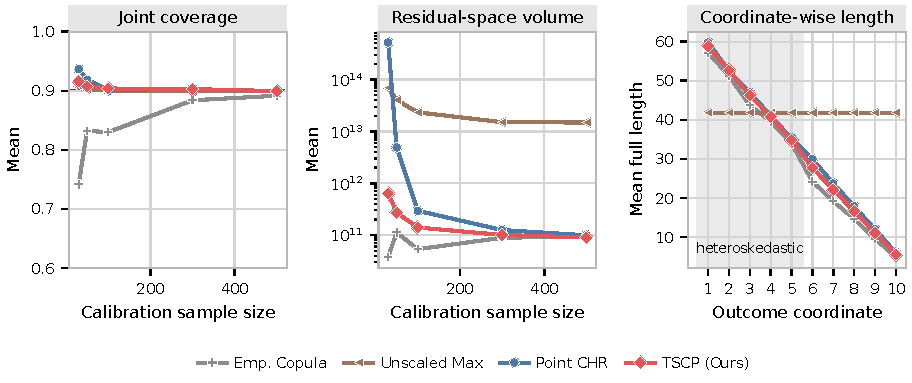
\includegraphics[width=0.94\textwidth]{figures/fig_body_partial_heteroskedasticity.pdf}
  \caption{Performance when only the first five of ten outcomes are
  heteroskedastic in $X_1$. The shaded coordinates in the right panel are the
  heteroskedastic ones; full interval lengths are shown for $n=100$. Results
  are averaged over 200 independent repetitions.}
  \label{fig:body-partial-hetero}
\end{figure*}

\subsection{Quantile-Regression Scores and CQHR}
\label{sec:cqr-experiments}

We next replace absolute mean-regression residuals with coordinate-wise CQR
scores. Let $\widehat q_{\ell,j}(x)$ and $\widehat q_{u,j}(x)$ denote fitted
lower and upper conditional quantiles. The signed score is
\[
  S_j(x,y)
  = \max\{\widehat q_{\ell,j}(x)-y_j,
           y_j-\widehat q_{u,j}(x)\}.
\]
Negative values correspond to observations strictly inside the base interval.
Because the current TSCP theory is stated for nonnegative scores, the primary
experiment uses the capped score $E_j=\max\{S_j,0\}$. This transformation can
only inflate the base interval and therefore avoids the overly conservative
absolute-value transformation. Unscaled Max and Emp. Copula use the raw signed
scores, while CQHR is applied in its native form.

We simulate $d=3$ Gaussian outcomes with noise scales $(3,2,1)$, fit separate
gradient-boosted quantile regressions using 2,400 training observations, and
evaluate on 600 test observations. Each quantile model uses 100 boosting
stages, maximum tree depth $5$, learning rate $0.05$, and minimum leaf size
$5$. The base-interval miscoverage is $0.5$ and
the final target miscoverage is $0.1$. Each of the 30 repetitions uses fresh
training, test, and calibration samples. Figure~\ref{fig:body-cqr} shows that
TSCP's empirical coverage fluctuates around the target, ranging from $0.899$
to $0.922$ over the displayed calibration sizes, while its mean outcome-space
volume remains between $2.62\times10^4$ and $3.62\times10^4$. CQHR attains
empirical coverage between $0.894$ and $0.909$ but is much larger and more
variable in this design; at $n=100$, its mean volume is
$1.29\times10^8$. This comparison is specific to the stated base
quantile models and is not a claim that one method uniformly dominates CQHR.
Base-interval and shifted-score sensitivity analyses are in
Appendix~\ref{app:cqr-sensitivity}.

\begin{figure*}[t]
  \centering
  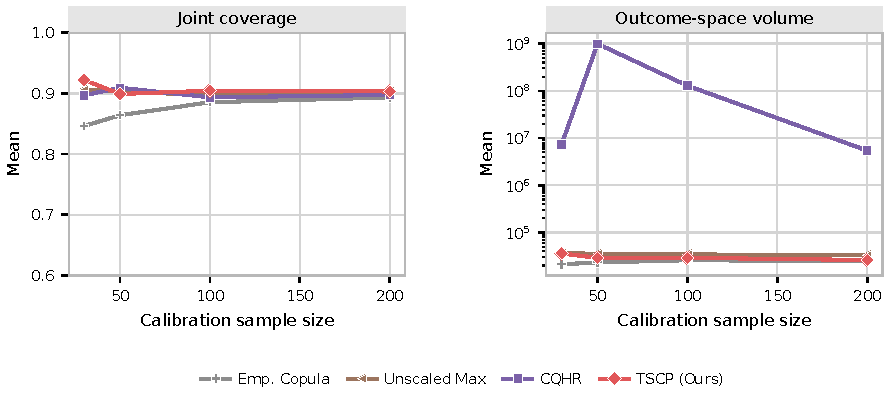
\includegraphics[width=0.88\textwidth]{figures/fig_body_cqr_comparison.pdf}
  \caption{CQR experiment with $d=3$ and base-interval miscoverage $0.5$.
  TSCP uses capped nonnegative scores, Unscaled Max and Emp. Copula use raw
  signed scores, and CQHR uses its native quantile-hyperrectangle
  construction. Results are averaged over 30 independent repetitions.}
  \label{fig:body-cqr}
\end{figure*}

Figure~\ref{fig:body-cqr-coordinate-bars} reports the corresponding
coordinate-wise comparison at $n=100$. TSCP's mean full lengths are
$(36.2,36.9,20.9)$, compared with $(33.3,33.8,29.0)$ for Unscaled Max and
$(46.2,120.5,66.9)$ for CQHR. In particular, TSCP preserves a substantially
shorter third-coordinate interval than Unscaled Max, while CQHR is much wider
on the second and third coordinates in this fitted-quantile design. As above,
the coordinate-wise lengths should be interpreted together with the joint
coverage panel rather than compared without regard to calibration.

\begin{figure*}[t]
  \centering
  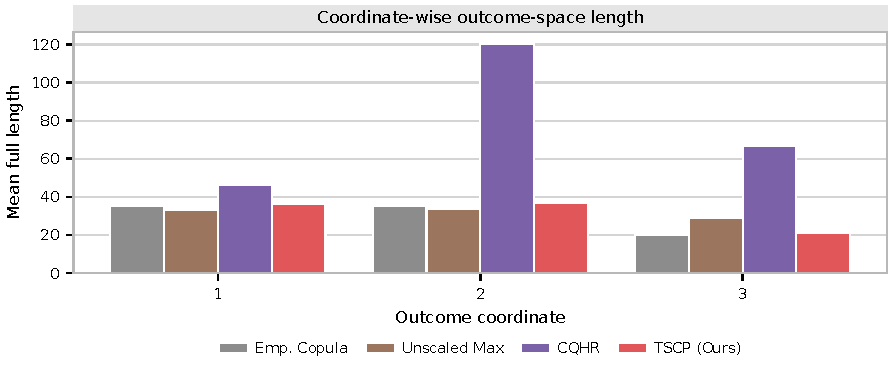
\includegraphics[width=0.82\textwidth]{figures/fig_body_cqr_coordinate_bars.pdf}
  \caption{Coordinate-wise mean full outcome-space lengths for the CQR
  experiment with $d=3$, $n=100$, base-interval miscoverage $0.5$, and final
  target coverage $0.9$. TSCP uses capped scores, Unscaled Max and Emp. Copula
  use raw signed scores, and CQHR uses its native construction. Results
  average 30 independent repetitions.}
  \label{fig:body-cqr-coordinate-bars}
\end{figure*}

\subsection{Real Data and Wall-Clock Runtime}
\label{sec:real-data-experiments}

We retain the six real-data benchmarks from the original experiments:
\texttt{stock}, \texttt{rf2}, \texttt{scm1d}, \texttt{scm20d},
\texttt{energy}, and \texttt{student}. Each result averages 200 random
training/calibration/test splits using proportions $75\%/5\%/20\%$. The
calibration sizes therefore range from $15$ on \texttt{stock} to $490$ on
\texttt{scm1d}. A multitask lasso is used for \texttt{stock}; random forests
are used for the other datasets. Table~\ref{tab:real-data} reproduces coverage
and residual-space volume for the four primary methods.

\begin{table*}[t]
\centering
\small
\begin{tabular}{llrrr}
\toprule
Dataset & Method & $d$ & Coverage & Volume \\
\midrule
\texttt{stock} & Unscaled Max & 6 & $0.940\,(0.057)$ & $6.03\mathrm{e}{-2}\,(1.57\mathrm{e}{-1})$ \\
 & Emp. Copula & 6 & $0.727\,(0.113)$ & $1.01\mathrm{e}{-5}\,(9.80\mathrm{e}{-6})$ \\
 & Point CHR & 6 & $1.000\,(0.000)$ & $\infty$ \\
 & \textbf{TSCP} & 6 & $0.956\,(0.059)$ & $\mathbf{1.86\mathrm{e}{-3}\,(8.55\mathrm{e}{-3})}$ \\
\addlinespace
\texttt{rf2} & Unscaled Max & 8 & $0.900\,(0.016)$ & $4.14\mathrm{e}{3}\,(2.90\mathrm{e}{3})$ \\
 & Emp. Copula & 8 & $0.893\,(0.016)$ & $5.35\mathrm{e}{1}\,(4.69\mathrm{e}{1})$ \\
 & Point CHR & 8 & $0.901\,(0.022)$ & $\mathbf{6.85\mathrm{e}{1}\,(7.55\mathrm{e}{1})}$ \\
 & TSCP & 8 & $0.901\,(0.017)$ & $5.42\mathrm{e}{2}\,(1.50\mathrm{e}{3})$ \\
\addlinespace
\texttt{scm1d} & Unscaled Max & 16 & $0.900\,(0.016)$ & $2.74\mathrm{e}{39}\,(4.02\mathrm{e}{39})$ \\
 & Emp. Copula & 16 & $0.893\,(0.016)$ & $1.09\mathrm{e}{39}\,(1.34\mathrm{e}{39})$ \\
 & Point CHR & 16 & $0.905\,(0.020)$ & $2.84\mathrm{e}{39}\,(5.43\mathrm{e}{39})$ \\
 & \textbf{TSCP} & 16 & $0.901\,(0.015)$ & $\mathbf{1.52\mathrm{e}{39}\,(2.61\mathrm{e}{39})}$ \\
\addlinespace
\texttt{scm20d} & Unscaled Max & 16 & $0.901\,(0.016)$ & $2.70\mathrm{e}{40}\,(2.92\mathrm{e}{40})$ \\
 & Emp. Copula & 16 & $0.892\,(0.017)$ & $1.18\mathrm{e}{40}\,(1.19\mathrm{e}{40})$ \\
 & Point CHR & 16 & $0.902\,(0.023)$ & $3.00\mathrm{e}{40}\,(8.00\mathrm{e}{40})$ \\
 & \textbf{TSCP} & 16 & $0.901\,(0.016)$ & $\mathbf{1.53\mathrm{e}{40}\,(1.50\mathrm{e}{40})}$ \\
\addlinespace
\texttt{energy} & Unscaled Max & 2 & $0.917\,(0.049)$ & $1.58\mathrm{e}{1}\,(6.80\mathrm{e}{0})$ \\
 & Emp. Copula & 2 & $0.886\,(0.061)$ & $5.41\mathrm{e}{0}\,(4.49\mathrm{e}{0})$ \\
 & Point CHR & 2 & $0.899\,(0.069)$ & $8.81\mathrm{e}{0}\,(2.42\mathrm{e}{1})$ \\
 & \textbf{TSCP} & 2 & $0.922\,(0.048)$ & $\mathbf{6.95\mathrm{e}{0}\,(4.43\mathrm{e}{0})}$ \\
\addlinespace
\texttt{student} & Unscaled Max & 3 & $0.904\,(0.055)$ & $\mathbf{1.51\mathrm{e}{2}\,(1.27\mathrm{e}{2})}$ \\
 & Emp. Copula & 3 & $0.861\,(0.073)$ & $1.08\mathrm{e}{2}\,(7.19\mathrm{e}{1})$ \\
 & Point CHR & 3 & $0.939\,(0.057)$ & $6.89\mathrm{e}{2}\,(1.07\mathrm{e}{3})$ \\
 & TSCP & 3 & $0.912\,(0.056)$ & $1.98\mathrm{e}{2}\,(1.77\mathrm{e}{2})$ \\
\bottomrule
\end{tabular}
\caption{Performance on real datasets, averaged over 200 random splits. One
standard deviation is reported in parentheses. Bold volume denotes the
smallest average volume among the methods with empirical coverage at or above
the target, up to Monte Carlo variation. The calibration sizes are 15, 384,
490, 448, 38, and 32 in the order shown.}
\label{tab:real-data}
\end{table*}

Figure~\ref{fig:body-real-runtime} provides the wall-clock comparison requested
by the reviewers. TSCP constructs a region in $0.74$--$7.46$ milliseconds on
these datasets. It is slower than the algebraically simpler Unscaled Max and
Point CHR implementations, but substantially faster than Emp. Copula on the
two $16$-dimensional SCM datasets, where Emp. Copula requires approximately
$95$--$118$ milliseconds. These measurements include the complete conformal
region construction but exclude fitting the shared regression model.

The infinite Point CHR volume on \texttt{stock} should not be interpreted as
an intrinsic failure of the method. With only $n=15$ calibration observations,
its additional split leaves too few observations for a finite $0.9$ conformal
quantile. A practitioner committed to Point CHR would allocate a larger
fraction of the data to its final calibration stage, at the cost of fewer
observations for model and scale estimation.

\begin{figure*}[t]
  \centering
  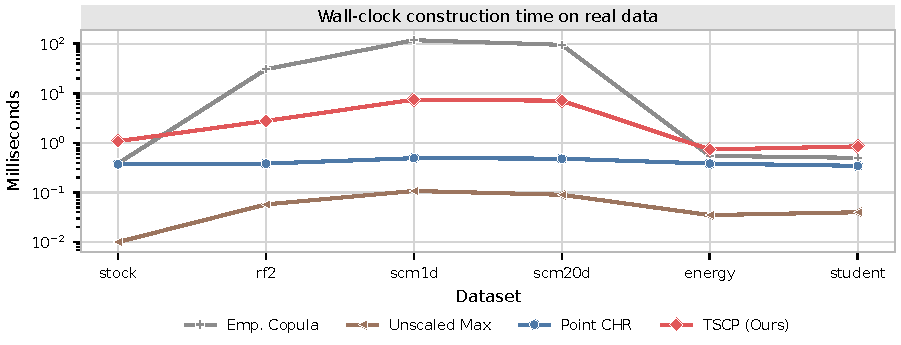
\includegraphics[width=0.90\textwidth]{figures/fig_body_real_runtime.pdf}
  \caption{Average wall-clock time for conformal region construction on the
  six real datasets. The vertical axis is logarithmic and reports
  milliseconds. All methods use the same fitted regression model in each
  split; model fitting and residual computation are excluded.}
  \label{fig:body-real-runtime}
\end{figure*}

\endgroup
